\documentclass[10pt,twocolumn]{article}

% ----------------------------------------------------------------------
% Posse: a general research paper on long-horizon agent-fleet management.
% Build: ~/.TinyTeX/bin/x86_64-linux/pdflatex POSSE_DESIGN (x2 for refs)
% ----------------------------------------------------------------------
\usepackage[T1]{fontenc}
\usepackage[utf8]{inputenc}
\usepackage{lmodern}
\usepackage{microtype}
\usepackage[margin=0.72in,columnsep=0.28in]{geometry}
\usepackage{graphicx}
\usepackage{xcolor}
\usepackage{booktabs}
\usepackage{array}
\usepackage{amssymb}
\usepackage{caption}
\usepackage{titlesec}
\usepackage{enumitem}
\usepackage[hidelinks]{hyperref}

\definecolor{posseNavy}{HTML}{20293B}
\definecolor{posseGold}{HTML}{B3841F}
\definecolor{posseSlate}{HTML}{5B6B86}
\definecolor{boxbg}{HTML}{F7F4EC}

\hypersetup{colorlinks=true, linkcolor=posseNavy, citecolor=posseNavy, urlcolor=posseGold}

\captionsetup{font=small,labelfont={bf,color=posseNavy},labelsep=period}
\setlength{\parindent}{1em}
\setlength{\columnsep}{0.28in}

\titleformat{\section}{\color{posseNavy}\large\bfseries}{\thesection}{0.6em}{}
\titleformat{\subsection}{\color{posseNavy}\normalsize\bfseries}{\thesubsection}{0.5em}{}
\titlespacing*{\section}{0pt}{1.4ex plus .3ex}{0.7ex}
\titlespacing*{\subsection}{0pt}{1.0ex plus .2ex}{0.5ex}

\newcommand{\yes}{{\color{posseNavy}\checkmark}}
\newcommand{\prt}{{\color{posseSlate}$\circ$}}
\newcommand{\no}{{\color{gray}\footnotesize$\times$}}
\newcommand{\code}[1]{\texttt{\small #1}}

\newcommand{\insight}[2]{%
  \par\vspace{0.6ex}\noindent\fcolorbox{posseGold}{boxbg}{%
  \parbox{0.955\columnwidth}{\small\textbf{\color{posseNavy}#1}\;#2}}\par\vspace{0.6ex}}

\title{\vspace{-3.2em}%
  \color{posseNavy}\bfseries\Large Posse: A Cost-Aware Operating System for\\[1pt]
  Long-Horizon, Human-Steered Fleets of LLM Agents\vspace{-0.2em}}
\author{\normalsize Anonymous Author(s)\\[-2pt]
  \small\textit{Affiliation withheld for review}}
\date{\small Under submission}

\begin{document}
\twocolumn[
\begin{@twocolumnfalse}
\maketitle
\vspace{-1.2em}
\begin{abstract}
\noindent
LLM agents are being deployed at rapid scale --- for software engineering, research,
data analysis, and business operations --- and increasingly they run not as a single
supervised task but as \emph{fleets} of agents operating continuously over long
horizons. This shift exposes a problem that agent frameworks, which optimize the
reasoning \emph{inside} one task, largely leave unsolved: how to \emph{use and manage
many agents efficiently} over time. Each agent's work must stay coherent across
interruptions and restarts, and many agents must be organized and steered
concurrently. The system must keep itself running and recover from failures; and,
because every token is billed and long-lived agents carry large contexts, cost must be
engineered as a deployment grows. We present \textbf{Posse}, an operating system for long-horizon
agent fleets, organized around seven requirements (R1--R7) that session-based
frameworks miss. Posse groups agents into user-defined \emph{precincts} whose durable,
bounded, auditable records form a \emph{shared} memory substrate --- a new or different
agent reads them to pick up a line of work cheaply, instead of the expensive habit of
keeping one agent alive for the whole horizon; runs each unit of work as a \emph{deputy}
whose identity survives process death; steers and interrupts deputies through an
asynchronous message channel; and supervises the whole fleet with a single always-on
\emph{Sheriff}. Four
principles carry the design: identity decoupled from process liveness, token cost
treated as a first-class scheduling resource, a zero-cost mechanical control plane
separated from paid model cognition, and memory externalized as a shared record rather
than a private context. From the last principle we derive a
provider-parameterized, cache-aware scheduling policy whose poll-versus-park break-even we
give in closed form. Posse is released as open source; the framework ships the Sheriff
and a Receptionist front desk, and users define the precincts that fit their domain.
\end{abstract}
\vspace{0.6em}
\end{@twocolumnfalse}
]

% ======================================================================
\section{Introduction}
% ======================================================================
Large language model (LLM) agents have moved rapidly from demonstrations to
deployment. Coding agents open pull requests and run for hours~\cite{openhands,claudecode};
research agents autonomously gather and synthesize sources~\cite{gptresearcher};
agents drive data analysis, customer operations, and multi-step business workflows. A
second shift is now underway: rather than one agent invoked for one task,
organizations run \emph{fleets} of agents --- many at once, over long horizons,
increasingly with little human attention. A fast-growing ecosystem reflects this ---
meta-harnesses that orchestrate and swap between agent backends~\cite{omnigent,exo},
secured runtimes that host third-party agents~\cite{nemoclaw}, and observability
platforms that trace and price them~\cite{langfuse,agentops}.

As deployments scale from one supervised session to many long-running agents, a
different problem dominates --- not how a single agent \emph{reasons}, but how to
\emph{use and manage a fleet efficiently} over time. Four practical difficulties
recur:
\begin{itemize}[leftmargin=1.1em,itemsep=1.5pt,topsep=2pt]
  \item \textbf{Continuity.} A line of work and its follow-ups must stay coherent
  across interruptions, restarts, and the death of the process that ran it.
  \item \textbf{Concurrency.} Many independent agents must be organized, owned, and
  steered without collapsing into an untraceable sprawl.
  \item \textbf{Autonomy.} The system must keep itself running --- routing work,
  staying alive, recovering from crashes and provider rate limits --- with no human
  babysitting a terminal.
  \item \textbf{Cost.} Because every token is billed and long-lived agents carry
  large contexts, cost must be engineered as the fleet grows, not discovered on the
  invoice.
\end{itemize}
This management layer is where real deployments strain, and it is largely outside what
today's agent frameworks address.

\noindent\textbf{Why existing systems fall short.} Each solves part of the picture and
leaves the rest to the application. Agent frameworks~\cite{langgraph,autogen,crewai,metagpt}
optimize the \emph{inside} of one task episode --- reasoning, tool use, division of
labor --- and assume a human is present for its duration. Meta-harnesses~\cite{omnigent,exo}
run and swap agent backends but do not manage a long-horizon fleet's identity,
recovery, or cost. Secured runtimes~\cite{nemoclaw,openhands} isolate and host agents
without durable cross-restart identity or a cost model. Observability
tools~\cite{langfuse,agentops,phoenix} \emph{watch} agents but do not \emph{manage}
them. Durable-execution engines~\cite{temporal,stepfns} give identity and
resume-across-crash to ordinary workflows, but have no notion of LLM \emph{token} cost,
bounded LLM \emph{memory}, or an absent human. No existing system covers the whole
management layer (\S\ref{sec:bg}).

\noindent\textbf{This paper.} We present \textbf{Posse}\footnote{The organizing
metaphor is a \emph{Sheriff} (a single autonomous system manager) supervising
\emph{Deputies} (ephemeral worker agents), grouped into \emph{Precincts} (domains).},
an operating system for long-horizon agent fleets. Posse distills the difficulties
above into seven requirements (R1--R7, \S\ref{sec:reqs}) and meets them with four
principles: (I1) a thread's identity is a durable \emph{record}, decoupled from any
live process; (I2) token cost is a first-class \emph{scheduling} resource; (I3) a
zero-cost mechanical control plane is separated from paid model cognition; and (I4)
memory is a shared, durable record rather than a private context. Concretely,
Posse organizes work into user-defined \emph{precincts} with durable, bounded memory;
runs each unit of work as an ephemeral \emph{deputy} whose identity outlives its
process; steers deputies through an asynchronous message channel that can interrupt
them mid-task; and supervises the whole fleet with a single always-on \emph{Sheriff}.
The framework ships only the Sheriff and a \emph{Receptionist} front desk; users define
the precincts that fit their domain.

\noindent\textbf{Contributions.}
\begin{enumerate}[leftmargin=1.3em,itemsep=1pt,topsep=2pt]
  \item A \emph{requirements analysis} (R1--R7) for long-horizon, human-steered
  agent-fleet management, and a comparison showing that popular systems --- built for
  supervised single episodes or for adjacent concerns --- cover it only partially
  (\S\ref{sec:bg}).
  \item Four design principles that resolve the tensions among the requirements
  (\S\ref{sec:overview}).
  \item A modular design realizing them --- precinct memory (\S\ref{sec:precincts}),
  deputy continuity (\S\ref{sec:deputies}), the control plane (\S\ref{sec:email}), the
  Sheriff (\S\ref{sec:sheriff}), cost-aware scheduling (\S\ref{sec:cost}), multi-agent
  coordination (\S\ref{sec:jtf}), and observability (\S\ref{sec:dash}) --- the core
  modules presented with the alternatives we considered and our rationale.
  \item An analytical, provider-parameterized \emph{cost-scheduling result}: a cache-TTL
  break-even that makes the poll-versus-park decision optimal, given in closed form and
  independent of context size (\S\ref{sec:cost}).
  \item An open-source implementation; the framework ships the Sheriff and Receptionist,
  and users create their own precincts.
\end{enumerate}

% ======================================================================
\section{Background and Requirements}
\label{sec:bg}
% ======================================================================

\subsection{The landscape}
Systems that touch agent management cluster into six families.

\noindent\textbf{(a) Autonomous single-agent loops.} AutoGPT and
BabyAGI~\cite{autogpt,babyagi} wrap one LLM in a plan--act--observe loop; reasoning
scaffolds --- ReAct~\cite{react}, Reflexion~\cite{reflexion}, Tree of
Thoughts~\cite{tot} --- improve its decisions. GPT-Researcher~\cite{gptresearcher}
autonomously plans and synthesizes a research report. These target the quality of one
agent's trajectory.

\noindent\textbf{(b) Multi-agent frameworks.} AutoGen~\cite{autogen},
CAMEL~\cite{camel}, MetaGPT/ChatDev~\cite{metagpt,chatdev}, and CrewAI~\cite{crewai}
run several role-specialized agents that converse or follow a standard procedure to
complete one project.

\noindent\textbf{(c) Graph / workflow orchestration.} LangGraph~\cite{langgraph}
and OpenAI's Swarm~\cite{swarm} are construction kits: a developer wires agents into a
stateful graph or hand-off routine that executes when invoked.

\noindent\textbf{(d) Meta-harnesses and runtimes.} A newer layer runs and secures
agents rather than authoring them. Omnigent~\cite{omnigent} orchestrates and hot-swaps
agent backends (Claude Code, Codex, Cursor, custom) behind one interface, with policy
and sandboxing; exo~\cite{exo} is a comparable agent harness. NemoClaw~\cite{nemoclaw}
and OpenHands~\cite{openhands} host and sandbox agents with managed inference and a
control surface. These make agents \emph{runnable and safe} but treat each run as
transient.

\noindent\textbf{(e) Observability.} Langfuse~\cite{langfuse},
AgentOps~\cite{agentops}, and Arize Phoenix~\cite{phoenix} trace, evaluate, and price
agent runs. They \emph{observe}; they do not \emph{drive} the fleet.

\noindent\textbf{(f) Durability and OS abstractions.} Durable-execution engines ---
Temporal~\cite{temporal}, AWS Step Functions~\cite{stepfns}, Airflow~\cite{airflow} ---
give ordinary workflows an identity that survives process death and resumes on an
event. AIOS~\cite{aios} proposes an ``LLM agent operating system'' kernel;
MemGPT~\cite{memgpt} manages context like virtual memory; server-side
threads~\cite{assistants} persist a conversation's state. These are the closest in
spirit to Posse and we return to them in \S\ref{sec:related}.

\subsection{Requirements}
\label{sec:reqs}
From the difficulties in \S1 plus the operational reality of a metered API, a finite
model window, and a human who cannot watch every agent, we distill seven requirements
for managing a long-horizon agent fleet.

\begin{description}[leftmargin=1.15em,itemsep=1pt,topsep=2pt,font=\normalfont\bfseries\color{posseNavy}]
  \item[R1 Long-horizon continuous operation.] Run unattended for days to weeks, not
  for one session.
  \item[R2 Durable thread identity \& continuity.] A line of work keeps one identity
  and its context \emph{across process death}.
  \item[R3 Concurrent fleet management.] Many independent threads, each isolated,
  owned, and navigable.
  \item[R4 Asynchronous human steering.] A human directs and \emph{interrupts} agents
  asynchronously, without holding a session open.
  \item[R5 Autonomous fault recovery.] Self-heal from crashes and provider rate limits.
  \item[R6 Cost-aware scheduling.] Treat token/\$ cost as a scheduled resource, not an
  afterthought.
  \item[R7 Bounded, shared, faithful memory.] What the fleet learns must outlive the
  process that learned it, be readable by \emph{any} agent, fit the model window when
  recalled, and come back as written, with its source --- not as an approximate
  reconstruction the agent must second-guess.
\end{description}
These are not fully orthogonal: R2, R3, and R7 are facets of one \emph{durable-record
substrate} (identity, ownership, shared memory), and R1 is unreachable without R5.
We list them separately because prior systems fail them \emph{independently} --- a
system can manage many threads (R3) yet lose each one's continuity on restart (R2).

\subsection{The gap, requirement by requirement}
\label{sec:gap}
The families above are strong in their own regimes, and several already meet R3's
concurrency half --- many units of work at once, though rarely as isolated, owned,
navigable threads. The rest of the list goes largely unmet, for reasons that split by
family. The families that build, run, or orchestrate agents treat each run as a
self-contained episode --- one task, one run, one project --- with a human close at
hand whenever input is needed; observability platforms are read-only by design; and
durable-execution engines run for months unattended, but over conventional code,
where windows, contexts, and token bills do not exist. Five failures follow.

\noindent\textbf{Identity dies with the process.} In most systems a ``thread'' is a
running object --- a process, a graph run, a chat --- so when the object ends, the
thread's identity and accumulated context end with it (fails R2). The loss is not
exotic. An analyst has an agent draft a report on Monday and on Thursday replies,
``now break it down by region''; real work arrives exactly this way, as a sequence of
follow-ups. But if Monday's process has exited, Thursday's reply lands on a
\emph{fresh} agent that knows nothing of the data sources, caveats, and choices behind
the draft, and the human must re-brief it with a hand-written summary that is
inevitably lossy. AutoGPT~\cite{autogpt}, CrewAI~\cite{crewai}, and
AutoGen~\cite{autogen} tie the thread to a run that ends with the task.
LangGraph~\cite{langgraph} can persist a run's state, but only if the application
holds the \code{thread\_id} and reloads it --- nothing routes a reply that arrives
days later back to that state on its own. Server-side threads~\cite{assistants}
persist the conversation itself, and durable-execution
engines~\cite{temporal,stepfns} the workflow --- but a persisted transcript is not a
routed thread: nothing watches for Thursday's reply, matches it to Monday's thread,
and relaunches an agent on it.

\noindent\textbf{What an agent learns is trapped in its session.} The same coupling
leaves knowledge stranded along with identity. Suppose agent A spends a long session
learning a domain's quirks: which tools are reliable, which apparent shortcuts
dead-end, what was tried and rejected. The next task in that domain gets a new
agent that knows none of it, and existing designs offer only unattractive ways to
pass the knowledge on. Replaying A's transcript violates R7's bounded-recall clause
--- and presumes the transcript was persisted at all. Keeping A alive for the whole
horizon violates it too: one context growing without bound, the very pathology a
finite window and a metered bill forbid. Bolting retrieval onto an external store
scales, but what it returns is whichever fragments similarity search surfaces --- the
lesson comes back piecemeal, never guaranteed whole, not as it was written. What a
domain's agents have learned should be a shared, reusable asset that any newcomer
picks up cheaply and can rely on. MemGPT~\cite{memgpt} comes closest by bounding a
single agent's context, and AIOS~\cite{aios} by managing per-agent memory in its
kernel, but per-agent memory is still trapped memory --- neither turns what one agent
learned into records \emph{any} agent can read (each meets R7 only in part).

\noindent\textbf{Steering assumes a waiting human.} In a fleet the human is absent by
design, but their feedback cannot wait for the next session. An agent forty minutes
into an expensive job may be working from a specification the human has since realized
is wrong; the correction is useful only if it reaches \emph{that} agent promptly and
redirects it \emph{without} discarding the forty minutes of computation already done.
Existing designs invert the relationship. LangGraph's \code{interrupt()} pauses the
run at a predetermined point and \emph{waits} for the human to supply input --- the
graph, not the human, decides when feedback may arrive. AutoGen likewise solicits
input inline, through a human proxy. In both, a correction arriving from outside the
script has no path into a run in flight; the operator's recourse is to stop the job
and restart it corrected --- forfeiting the very computation the correction was meant
to save. Temporal narrows the gap: a signal is durable and needs no live worker
process. But it must name a still-open workflow
execution~\cite{temporal}, and what it updates is the program's state --- redirecting
an agent means reaching its \emph{reasoning}, folding the correction into a context
mid-flight, which no workflow signal models (meets R4 for code, not for agents).

\noindent\textbf{Nothing keeps the fleet alive.} Over a horizon of weeks, the routine
failures of a shared, pay-per-token deployment are a certainty rather than a tail
risk: the
provider's weekly rate limit trips at 2\,a.m., the machine reboots, a process is
OOM-killed. Without recovery, the affected work silently stalls until a human notices
--- perhaps not until morning --- and a fleet that needs a minder is not autonomous
in any useful sense. Agent frameworks retry a failed tool \emph{call} inside a run
--- LangGraph attaches retry policies to graph nodes~\cite{langgraph} --- and
durable-execution engines~\cite{temporal,stepfns} restart crashed \emph{workflows}.
Secured runtimes~\cite{nemoclaw,openhands} host the agent's process and will restart
a dead container, but leave rate-limit-aware detection and timing to the application.
None treats the agent's \emph{process} as the thing to supervise: noticing that it
has died or been rate-limit-blocked, then relaunching it --- immediately after a
crash, at the reset after a limit. Durable engines earn their R1 and R5 for what they
run; nothing yet extends either to the agent's own process.

\noindent\textbf{Cost is observed, never scheduled.} At fleet scale the dominant cost
is \emph{touching} large contexts, and whether each touch is a warm cached read or a
cold full-context rewrite is decided by scheduling rather than by model choice.
Consider a fleet whose agents each wait on hour-long jobs, checking progress every few
minutes: a check that lands after the short cache window rewrites the \emph{entire}
context at roughly $12.5\times$ the price of a cached read (one major provider's
published caching prices~\cite{promptcache}), so a cadence only slightly too slow can
quietly multiply that fleet's monthly bill by an order of magnitude. Observability
tools~\cite{langfuse,agentops} \emph{measure} this spend after the fact, and
AIOS~\cite{aios} schedules LLM calls for latency rather than for tokens, but no
orchestration framework we surveyed \emph{schedules} the poll-versus-park decision ---
keep the context warm, or sleep until an event wakes the agent --- against the
provider's cache economics (fails R6; \S\ref{sec:cost} derives the break-even).

\begin{table*}[t]
\centering
\caption{\textbf{Design emphasis} in the long-horizon fleet-management regime of
\S\ref{sec:reqs} --- \emph{not} a quality ranking; each system excels in the regime it
targets. Rubric: \yes\ = a first-class system property; \prt\ = partial, or present but
left to the application; \no\ = not a concern of the design. Cells reflect each system's
\emph{default, first-class} stance, not what is achievable with custom code. ``Cost
\emph{sched.}'' is cost-aware \emph{scheduling}, distinct from the cost \emph{tracking}
that observability tools do well.}
\label{tab:compare}
\small
\renewcommand{\arraystretch}{1.15}
\setlength{\tabcolsep}{2.5pt}
\begin{tabular}{@{}l l ccccccc@{}}
\toprule
 & \textbf{Type} & \textbf{R1} & \textbf{R2} & \textbf{R3} & \textbf{R4} & \textbf{R5} & \textbf{R6} & \textbf{R7}\\
 & & \scriptsize horizon & \scriptsize identity & \scriptsize fleet & \scriptsize async H-in-loop & \scriptsize recovery & \scriptsize cost \emph{sched.} & \scriptsize LLM memory\\
\midrule
AutoGPT / BabyAGI~\cite{autogpt,babyagi}      & auton.\ loop         & \prt & \no  & \no  & \no  & \no  & \no  & \prt \\
ReAct / Reflexion~\cite{react,reflexion}      & reasoning loop       & \no  & \no  & \no  & \no  & \no  & \no  & \prt \\
GPT-Researcher~\cite{gptresearcher}           & research agent       & \prt & \no  & \no  & \no  & \no  & \no  & \prt \\
AutoGen~\cite{autogen}                        & multi-agent chat     & \no  & \no  & \prt & \prt & \no  & \no  & \no  \\
CrewAI / MetaGPT~\cite{crewai,metagpt}        & role crew / SOP      & \no  & \no  & \prt & \no  & \no  & \no  & \no  \\
LangGraph~\cite{langgraph}                    & graph orchestration  & \prt & \prt & \prt & \prt & \prt & \no  & \prt \\
Omnigent~\cite{omnigent} / exo~\cite{exo}     & meta-harness         & \prt & \prt & \yes & \prt & \prt & \no  & \no  \\
NemoClaw~\cite{nemoclaw} / OpenHands~\cite{openhands} & secured runtime & \prt & \prt & \prt & \prt & \prt & \no  & \prt \\
Langfuse / AgentOps~\cite{langfuse,agentops}  & observability        & \no  & \no  & \prt & \no  & \no  & \prt & \no  \\
Durable exec.\ (Temporal)~\cite{temporal,stepfns} & workflow engine  & \yes & \yes & \yes & \prt & \yes & \no  & \no  \\
AIOS / MemGPT~\cite{aios,memgpt}              & agent OS / memory OS  & \prt & \prt & \prt & \no  & \prt & \prt & \prt \\
\midrule
\textbf{Posse (this work)}                    & \textbf{agent ops}   & \yes & \yes & \yes & \yes & \yes & \yes & \yes \\
\bottomrule
\end{tabular}
\end{table*}

Table~\ref{tab:compare} maps where each design puts its effort. Durable-execution
engines come closest on identity and recovery, but what they make durable is
\emph{compute} --- code state, not an agent's context --- and their model has no
notion of a token bill. The gap Posse targets is the \emph{conjunction}: asynchronous
steering (R4), scheduled cost (R6), and shared, faithful memory (R7), on a substrate
that gives agent threads durable identity (R2), ownership and navigability at fleet
scale (R3), and process-level supervision (R1, R5) --- while reusing the reasoning
and multi-agent ideas of families (a)--(c) \emph{inside} its deputies, the
harness/runtime ideas of (d) to run them, observability's read-only view (e) as its
dashboard, and the OS/memory stance of (f) in its precinct records. One \yes\ in the
Posse row warrants a word. On R2 the design hands the user a \emph{continuity dial}
per \emph{case}, Posse's term for one thread of work; the dial currently has two
settings. Replying to a case, even a finished one, relaunches its original deputy on
its recorded session, identity and context intact. Opening a new case gets a fresh
deputy briefed from the durable records. Only the cost-aware policy that would set
the dial automatically remains future work (\S\ref{sec:deputies}).

% ======================================================================
\section{Design Overview}
\label{sec:overview}
% ======================================================================

\subsection{Four principles}
The requirements pull against each other. Full continuity (R2) wants one long-lived
context; cost (R6) and the finite window punish exactly that. Autonomy (R1, R5) wants
always-on processes; always-on-ness is what a naive design bills you for. Shared
knowledge (R7) wants to accumulate inside one agent's context, where it is neither
durable nor legible to a second agent. Posse rests on four decisions.

\insight{I1. Decouple identity from liveness.}{A thread's identity is a \emph{durable
record}, not a running process. Continuity (R2) is provided by persisted per-thread
records and a lineage map, so a thread can be resumed --- or rebuilt into a fresh
process under the same identity --- long after its original process died.}

\insight{I2. Make token cost a first-class scheduling resource.}{Every waiting
decision (poll vs.\ sleep), memory decision (keep vs.\ compact), and model choice
(cheap vs.\ capable) is taken against an explicit cost model derived from the
provider's cache economics (R6). Cost is scheduled, not discovered on the invoice.}

\insight{I3. Separate zero-cost mechanical control from paid cognition.}{The control
plane --- routing, liveness, recovery, waking, resource serialization, compaction
\emph{triggers} --- makes \emph{no} LLM calls. The model is invoked only for actual
work and a handful of manager decisions. This is what makes always-on operation (R1)
affordable (R6).}

\insight{I4. Treat memory as a shared record, not a private context.}{Knowledge that a
naive design traps inside one long-lived context --- legible only while that process,
and its bill, stays alive --- is instead externalized into per-precinct durable records
(R7): a compacted ledger, an append-only case log, and per-case files. Every deputy
reads them at spawn, so handing context to a second agent costs a file read rather than
a kept-alive session. Continuity becomes a property of the \emph{precinct}, not of any
one agent: any deputy can pick up where another left off.}

\subsection{System overview}
Figure~\ref{fig:arch} shows the result. Work is organized into \textbf{precincts} ---
user-defined domains (e.g.\ evaluation, development, research, operations). The
framework ships only a \emph{Receptionist} front desk and the \emph{Sheriff}; a user
creates whatever precincts fit their work. Each precinct owns durable \emph{records}: a
compacted \emph{ledger} (big-picture digest), an append-only \emph{case log} (index of
finished work), and per-thread \emph{case files} (\S\ref{sec:precincts}). We
distinguish a \emph{thread} --- the durable identity of a line of work --- from a
\emph{case} --- one numbered unit of work on it; a thread is a sequence of cases. Each
case is worked by a \textbf{deputy}: an ephemeral LLM worker that lives for one case,
messages the human a plan/milestones/result, and closes the case by appending to the
records (\S\ref{sec:deputies}).

The human steers through an \textbf{asynchronous message channel} (our implementation
uses email; Fig.~\ref{fig:arch}, top). An always-on \emph{router} maps each message
--- mechanically, no LLM --- to an existing thread (a reply), a new deputy in a tagged
precinct, or the Receptionist (\S\ref{sec:email}). Overseeing everything is the
\textbf{Sheriff} (left): a single system manager that supervises deputy liveness and
precinct-records health. Its monitoring is zero-API (I3); it spends tokens only to
compact a ledger or decide a deputy's change-request. Underneath sit always-on daemons
that route, relaunch, event-wake, and serialize contended resources; a read-only
\textbf{dashboard} (right) observes it all. The ``operating system'' framing is literal
in the classic-services sense: the cost-aware wait policy (\S\ref{sec:cost}) is the
\emph{scheduler}, ledger compaction (\S\ref{sec:precincts}) is memory \emph{paging}, the
active-deputies board is the \emph{process table}, and the Sheriff is the process
\emph{supervisor} --- a mapping AIOS~\cite{aios} argues for in the abstract and Posse
supplies as a running system.

\begin{figure*}[t]
\centering
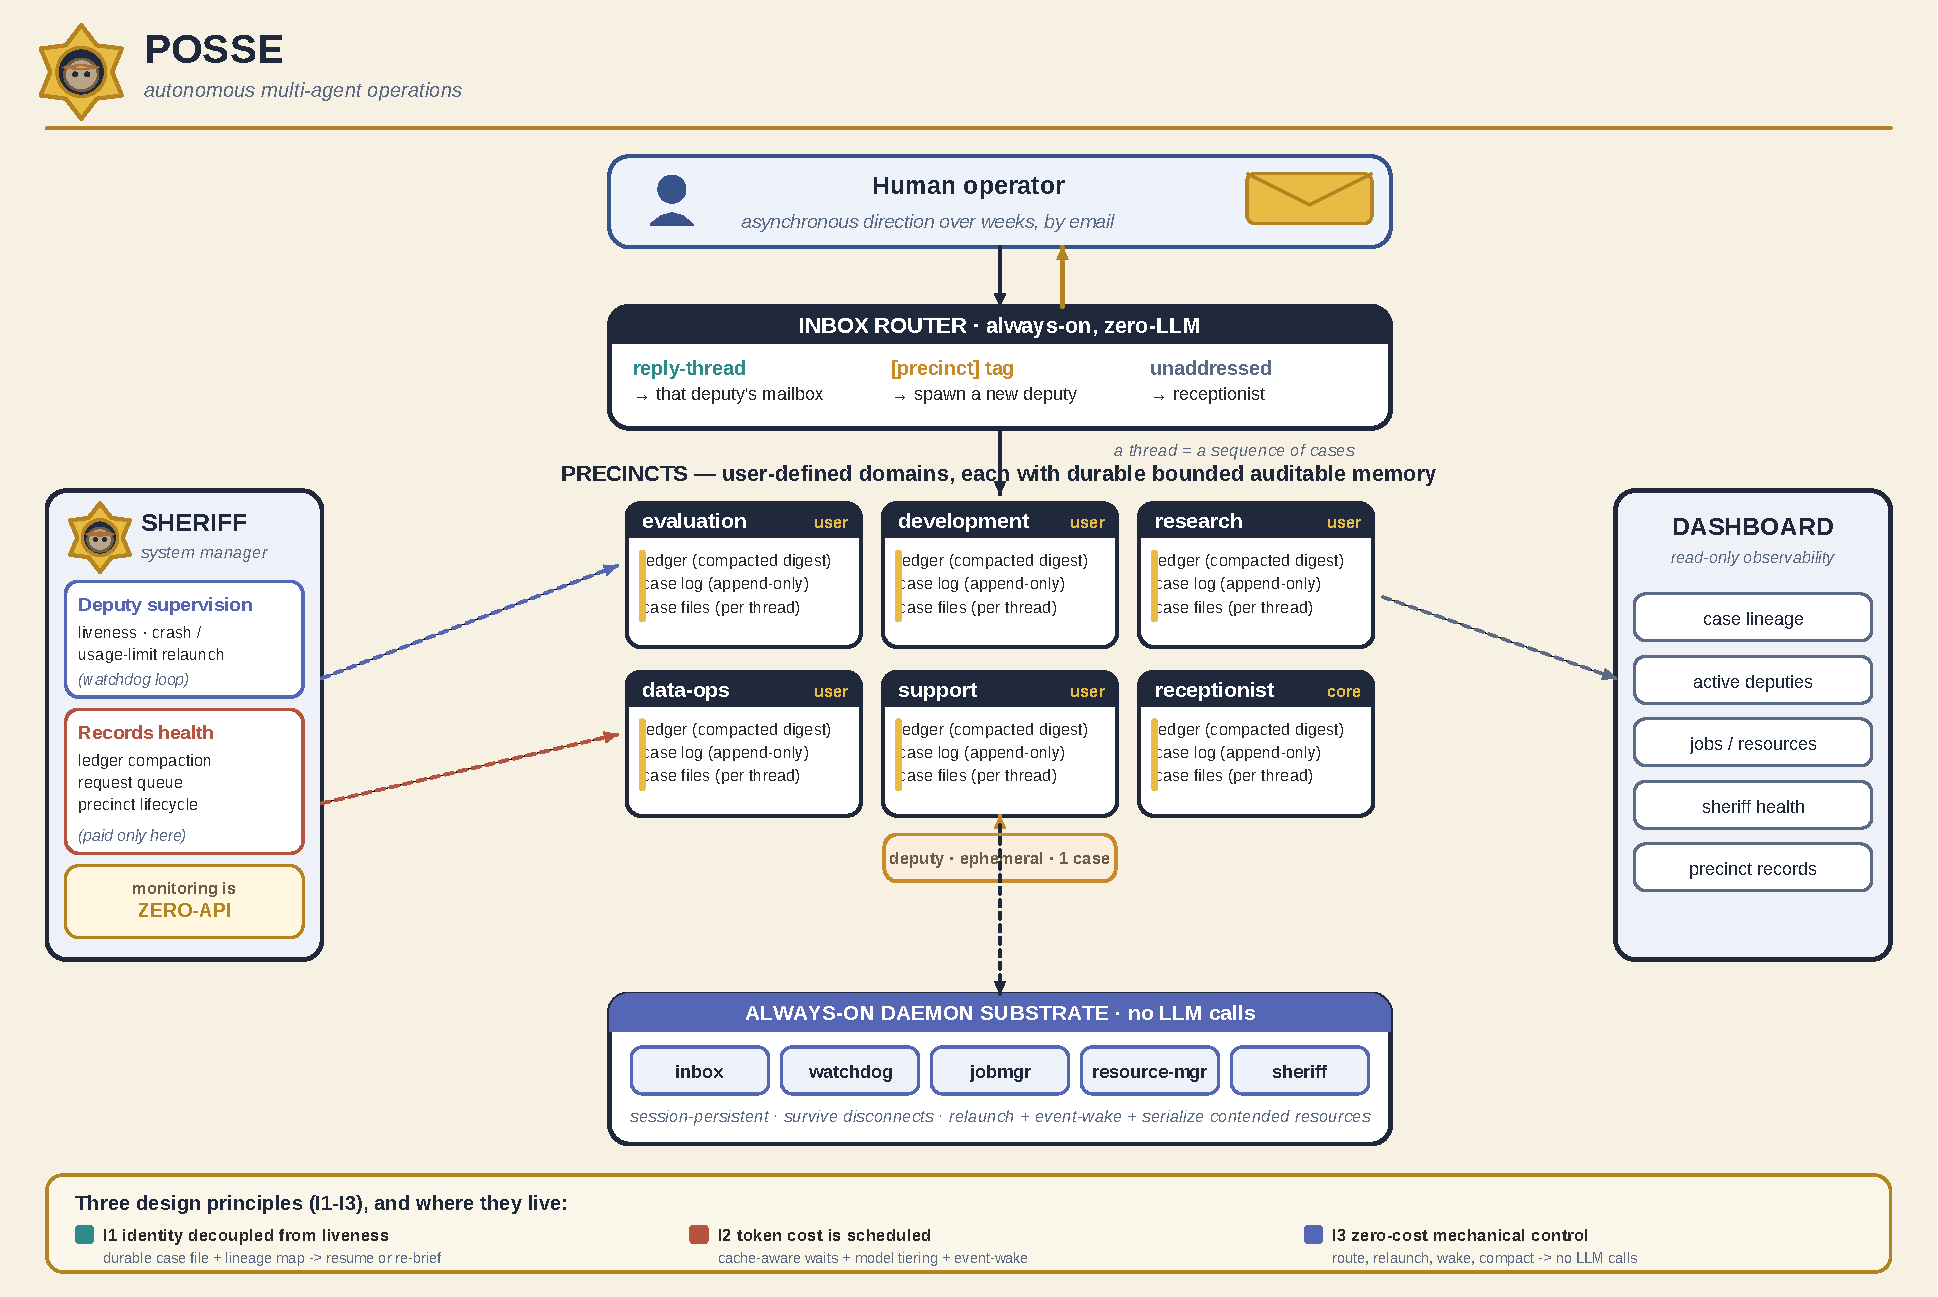
\includegraphics[width=0.98\textwidth]{fig/fig_architecture.pdf}
\caption{The Posse architecture. Work flows down the center (human $\to$ message
channel $\to$ router $\to$ user-defined precincts $\to$ deputies), with the always-on
daemon substrate underneath. The \emph{Sheriff} (left) manages the fleet with zero-API
monitoring, spending tokens only on ledger compaction and change-request decisions; the
\emph{dashboard} (right) observes read-only. The framework ships only the Sheriff and
Receptionist; the other precincts are illustrative and user-created.}
\label{fig:arch}
\end{figure*}

\subsection{Life of a case}
Figure~\ref{fig:life} traces one case. A message arrives and is routed; a deputy is
spawned or an existing identity resumed. At spawn the deputy is handed its precinct's
\emph{ledger} --- injected into its opening context --- so it starts already knowing the
domain's big picture and the state of related work (I4), rather than rediscovering it.
The deputy messages a plan, works in small
chunks, offloads compute to a detached job, and --- for a long job --- \emph{submits it
to a job manager and sleeps}, to be woken by an event rather than by polling
(\S\ref{sec:cost}). If the human replies mid-case, the deputy is \emph{surgically
interrupted}: its process is killed and relaunched with the new message injected, while
its detached jobs keep running (\S\ref{sec:email}); on resume it reads its mailbox
\emph{first}. Finally it reports a result and \emph{closes} the case: one ledger
paragraph, one case-log line, and a done-marker. Continuity (the dashed band) is carried
not by the process --- which may have died and been replaced --- but by the durable case
file and a resume-or-reinject decision (\S\ref{sec:deputies}). Underneath, the Sheriff
and daemons keep the deputy alive and wake it, with no LLM call.

\begin{figure*}[t]
\centering
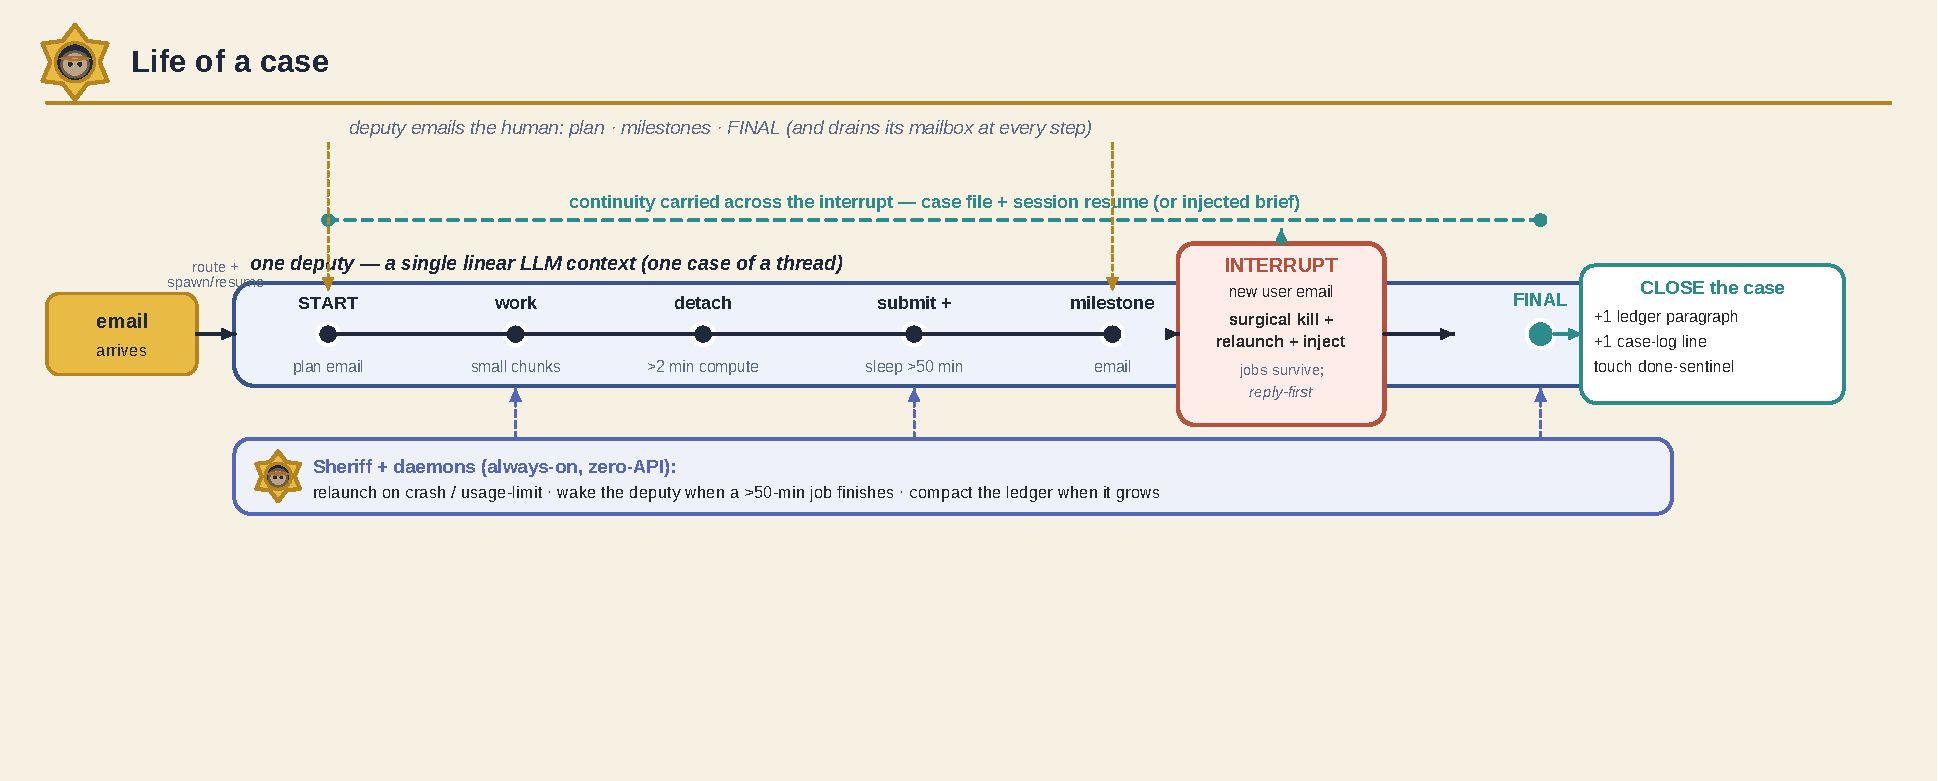
\includegraphics[width=0.98\textwidth]{fig/fig_lifecycle.pdf}
\caption{Life of a case. A deputy is one linear LLM context. Continuity survives the
interrupt (top dashed band) via the durable case file plus session resume or an injected
brief; the always-on Sheriff/daemon layer (bottom) relaunches, event-wakes, and compacts
--- with no LLM calls.}
\label{fig:life}
\end{figure*}

The remaining sections detail each module: what it does, the alternatives, and why we
chose as we did.

% ======================================================================
\section{Precincts and Bounded Memory}
\label{sec:precincts}
% ======================================================================
\textbf{Role (R7, R2, R3).} A precinct is a user-defined domain with durable,
structured memory. Its three record types form a hierarchy from most- to
least-compacted: a \emph{ledger} (a bounded big-picture digest, rewritten by compaction
as it grows), an append-only \emph{case log} (one line per finished case, never
rewritten, so attribution stays honest), and \emph{case files} (the full per-thread
record, the source of truth a resumed thread reads). All access goes through one
concurrency-safe records manager, never raw files --- the deliberate choke point that
enforces the append-only contract: a deputy may only \emph{append} (one ledger
paragraph and one case-log line, at close); only the Sheriff may compact, retract, or
create/delete a precinct.

\insight{Cheap memory sharing, without a long-lived agent.}{This is the payoff of
externalizing memory into precinct records. In the usual pattern, knowledge accrues
\emph{inside} one agent's long session: a \emph{different} agent cannot reuse it, and
keeping that agent alive for the whole horizon is expensive (its context grows without
bound). Posse decouples the two. A deputy may still take a sequence of follow-up cases
(the classic ``one long session''), but that is no longer the \emph{only} carrier of
knowledge: because every case's outcome is distilled into the shared ledger, log, and
case files, \emph{any} agent --- the same deputy on a follow-up, or a brand-new one, or
one in another concurrent thread --- acquires the precinct's accumulated context by
\emph{reading} it. Knowledge transfer costs a bounded read, not a kept-alive session ---
turning ``share what this agent learned'' from an ad-hoc, expensive operation into a
first-class, cheap one (R7, R2, and the cost side of R6).}

\insight{Framework ships empty of domains.}{Only the Sheriff and Receptionist are
built in. A user creates precincts for their own work --- evaluation, development,
research, whatever fits --- each with its own memory and default model. Precincts are
thus the unit of both \emph{organization} and \emph{extension}.}

\noindent\textbf{Design alternatives for long-term memory.} The crux is R7 versus the
model window and R6:
\begin{enumerate}[leftmargin=1.3em,itemsep=1pt,topsep=2pt]
  \item \emph{One growing context per domain.} Maximal continuity, but the context
  grows without bound, eventually exceeds the window, and --- per I2 --- becomes the
  most expensive thing to touch.
  \item \emph{Per-episode memory only.} Cheap and bounded, but forgets between cases;
  every follow-up is re-briefed by hand (fails R2, R7).
  \item \emph{Index all past work and fetch the most relevant snippets on demand}
  (similarity search over stored text). Scales to unbounded history, but a query returns
  a best-guess subset rather than the whole picture --- so it can silently miss relevant
  context --- and the index is not something a human can read to answer ``what does this
  domain know?''
  \item \textbf{Chosen: a compacted ledger + append-only log + full case files},
  managed by a separate zero-cost process. The ledger stays within a token budget
  (bounded, cheap to load); nothing is silently lost, because the log and case files
  are never compacted away; and the whole thing is plain text a human can read.
  Compaction (an LLM ``reflection'' over the domain, \S\ref{sec:sheriff}) is a coarse,
  operations-level analog of MemGPT's paging~\cite{memgpt} and Generative Agents'
  reflection~\cite{genagents}, but performed by the manager, not the worker, at domain
  granularity.
\end{enumerate}
Each precinct also carries a \emph{default model} (a capable model for most work, a
cheaper-but-capable model for token-heavy domains), so cost/capability tiering is a
per-domain policy (\S\ref{sec:cost}).

% ======================================================================
\section{Deputies and Thread Continuity}
\label{sec:deputies}
% ======================================================================
\textbf{Role (R2).} A deputy is an ordinary tool-using LLM agent that owns \emph{one
case}. The hard part is not what it does but how its \emph{thread} survives everything
that happens to the process running it.

\noindent\textbf{The failure to avoid.} The tempting design ties a thread's identity to
its process: a worker that finishes ends its session, so the next follow-up cannot find
it alive and spawns a brand-new worker with a fresh name and blank context, re-briefed
by a hand-written spec. Iterated over a fleet, this accumulates one throwaway identity
per task and scatters a single project across many differently-named agents ---
continuity tied to \emph{process liveness} rather than to the work.

\insight{The principle (I1).}{Route every follow-up to a \emph{stable, meaningful
identity} recorded in a persisted map --- not to whatever process happens to be alive.
That identity can be continued two ways: \code{resume} the \emph{same} live session
(full context, warm cache, maximal continuity), or spawn a fresh process under the
\emph{same} identity with a compact brief injected (prior case numbers, keywords,
pointers to the transcript and deliverables). Identity is stable either way; which
continuation applies is a \emph{steerable policy choice} about how much continuity the
task needs (below), never a side effect of which process happens to be alive.}

\noindent\textbf{Design alternatives (continuity policy).} We considered five points on
the continuity--cost spectrum:
\begin{enumerate}[leftmargin=1.3em,itemsep=1pt,topsep=2pt]
  \item[A.] \emph{Reuse-if-alive, else new agent.} Simplest and naturally parallel, but
  continuity is accidental and naming is chaotic.
  \item[B.] \emph{Standing domain agents} (never die). Strong continuity, one identity
  per domain, but one unbounded context: window pressure, cross-task interference,
  serialization.
  \item[C.] \emph{Per-thread persistent agent} (resume the exact session on demand).
  Precise continuity and a stable identity, but inherits B's unbounded growth on long
  threads.
  \item[D.] \emph{Fresh agent per task + injected context.} Always bounded and cheap,
  lineage explicit, but the injected brief is a summary, not the live session, and
  naming multiplies unless paired with a stable name.
  \item[E.] \textbf{Chosen direction: hybrid.} A stable per-thread \emph{name} (like
  C/D) plus a \emph{continue-or-reinject} choice --- resume the same session (C) when a
  task needs strong continuity, or spawn fresh under the same name with an injected brief
  (D) otherwise --- with the map persisted at creation. Among the five, only E avoids a
  \emph{severe} weakness on continuity, identity, and cost.
\end{enumerate}

\insight{Who decides: continuity vs.\ cost.}{The continue-or-reinject choice is
\emph{steerable}, not a fixed automatic threshold. Today the signal is mechanical --- a
threaded reply resumes the live session, a new case starts fresh under the same identity
(\S\ref{sec:email}) --- and the design extends this so the \emph{user} can require that a
hard, tightly-coupled task stay in one continuous session and the \emph{deputy} can flag
that its case needs the live context; an \emph{automatic} cost-threshold that sets the
dial without being told remains future work (\S\ref{sec:reqs}). Absent a stated need, the
default favors the bounded, cost-efficient path --- a fresh process under the same
identity with a compact brief. The philosophy: spend on strong continuity exactly where
the task genuinely needs it, and stay cheap everywhere else.}

% ======================================================================
\section{The Control Plane}
\label{sec:email}
% ======================================================================
\textbf{Role (R4).} The human steers the fleet through an \emph{asynchronous message
channel}, which is also the \emph{interrupt} mechanism. We chose an ordinary mailbox
(email in our implementation) deliberately: it is asynchronous by nature (the human is
never blocked and never blocking), durable (the mailbox is the queue), it threads (a
reply carries its lineage), and it needs no bespoke client.

\noindent\textbf{Routing.} An always-on router maps each message to its destination
\emph{mechanically} --- zero-LLM (I3) --- on two signals: (1) a reply threaded to a
deputy's earlier message $\to$ that deputy's \emph{mailbox}; (2) an explicit
\code{[precinct]} tag $\to$ a new deputy in that precinct (a reply to an
already-\emph{dead} deputy is attributed to its precinct via the persisted lineage
map). Only genuinely \emph{unaddressed} messages reach the Receptionist, whose
disposition (answer, or write a spec and spawn a deputy) is the one routing path that
spends an LLM turn. Deterministic routing on these two signals is cheap, predictable,
and cannot mis-route under ambiguity.

\noindent\textbf{Interruption.} When a reply targets a \emph{live} deputy, the message
is appended to its mailbox under a lock and the deputy is \emph{surgically interrupted}:
only its LLM process is killed and immediately relaunched with the mailbox injected;
its detached compute jobs --- separate processes --- keep running and are reconciled on
resume. On \emph{any} resume the deputy's first action is to drain its mailbox and reply
(the ``reply-first'' rule), so human feedback is never processed on a stale plan. The
delivery guarantee is \emph{at-least-once with an idempotent drain}: the append and a
boot marker are flock-serialized, so a burst of replies is drained \emph{together} on
the next boot rather than lost or double-processed, and a job that finishes
\emph{during} the interrupt window is reconciled from its result file on resume, never
re-submitted.

\noindent\textbf{Design alternatives.}
\begin{itemize}[leftmargin=1.1em,itemsep=1pt,topsep=2pt]
  \item \emph{Kill everything vs.\ surgical kill.} Killing the whole session would kill
  in-flight compute jobs (potentially hours of work). We kill only the agent process
  and let jobs survive as reconcilable orphans --- the single most important robustness
  property of the interrupt path.
  \item \emph{Debounce vs.\ immediate.} We interrupt \emph{immediately} on every human
  message, with boot-marker coalescing so a burst is drained together. Feedback latency
  matters more than avoiding a few extra relaunches.
\end{itemize}

% ======================================================================
\section{The Sheriff: Autonomous System Management}
\label{sec:sheriff}
% ======================================================================
\textbf{Role (R1, R5, R7).} The Sheriff is the fleet's single ``manager'' \emph{role},
presented as one but implemented as two cooperating always-on loops: a
\emph{deputy-supervision} loop (liveness monitoring --- crash and rate-limit recovery)
and a records daemon (precinct-records health --- ledger compaction, a change-request queue, precinct
lifecycle). We unify the \emph{model} (one manager, one dashboard panel) while keeping
the two proven loops physically separate; folding them into one process is a deferred
option.

\insight{The hard guarantee (I3).}{The Sheriff's \emph{monitoring is zero-API}. It
scans markers, process liveness, and ledger token-lengths mechanically; it makes an LLM
call \emph{only} to (a) compact a ledger that crossed its soft limit, or (b)
approve/deny a deputy's change-request. An idle pass costs nothing. This is what lets
the manager run forever without being a cost center.}

\noindent\textbf{Compaction.} When a ledger crosses a soft token budget the Sheriff
compacts it toward a target with one LLM call on a cheap model, given whole-system
context (all precincts' ledgers) and a fixed prompt that forbids inventing or silently
dropping a case. On a failure or rate limit it does \emph{not} truncate mechanically; it
waits and retries. The two outcomes are asymmetric: a ledger sitting slightly over
budget for a while costs almost nothing, whereas a rushed, low-quality compaction that
drops or garbles a case is expensive and hard to undo. The soft budget is a
\emph{trigger}, not a hard ceiling, so tolerating a brief overage while a good
compaction succeeds is the safe trade. The ledger is therefore \emph{bounded in normal
operation}, not unconditionally: a \emph{sustained} provider outage lets it grow past
budget until compaction next succeeds --- a temporarily larger ledger, never a lost case
(the never-compacted case log is the durable record). Compaction is the system's
``reflection'' step --- performed by the manager, off the worker's critical path.

\noindent\textbf{Change-requests \& authority.} Records mutations that are not simple
appends (retract a log line, edit a ledger, allocate an identifier, create/delete a
precinct) are \emph{sheriff-only}. A deputy requests them via a queue; the Sheriff
verifies the requester by matching its \code{(deputy, session)} against a live registry
--- the session token minted at spawn \emph{is} the shared secret, so a forged deputy is
rejected \emph{before} any LLM call --- then decides with one LLM call returning strict
JSON, performs the op, and journals it. A failed or rate-limited decision \emph{defers}:
it never auto-approves and never deletes by default. Destructive operations add gates:
deleting a precinct requires no active deputies, a confirmation reply matched
\emph{mechanically} by the zero-API daemon, and a recoverable trash window before hard
purge.

\noindent\textbf{Design alternatives.}
\begin{itemize}[leftmargin=1.1em,itemsep=1pt,topsep=2pt]
  \item \emph{On a failed compaction: truncate mechanically, or wait and retry?} We wait
  and retry. A ledger briefly over budget is cheap; a bad compaction that loses a case is
  expensive --- so we never trade compaction quality for a hard bound the soft budget
  does not actually require.
  \item \emph{Who may edit records?} Concentrating all non-append authority in one
  identity, gated by verified requests and a journal, keeps the record trustworthy;
  letting deputies edit their own history would destroy attribution.
\end{itemize}

% ======================================================================
\section{Cost-Aware Scheduling}
\label{sec:cost}
% ======================================================================
\textbf{Role (R6).} This is where Posse most departs from prior systems: \emph{token
cost is scheduled}, against a model of the provider's cache economics.

\noindent\textbf{Background: prompt caching.} Modern LLM providers cache the
\emph{prefix} of a request so that a later call sharing that prefix skips recomputing it.
The cache entry has a short time-to-live (TTL): a call that reuses a still-live prefix
pays a discounted \emph{cache-read} rate for those tokens, while a call that arrives
after the entry expired must re-establish the prefix at the full \emph{cache-write} rate.
The two rates differ sharply, and it is their \emph{ratio}, not the absolute price, that
a scheduler must reason about. For example, on Anthropic's Claude models a short (5-minute)
TTL cache \emph{write} is priced at $1.25\times$ the base input-token rate and a cache
\emph{read} at $0.1\times$~\cite{promptcache}, so re-establishing an expired prefix costs
$m \approx 12.5\times$ what reusing a live one does. The exact constant is
provider- and model-specific --- OpenAI publishes a comparable read
discount~\cite{openaicache} --- but every major provider exposes some version of this
cheap-read / expensive-rewrite gap; Posse is built for the general shape, not one price
list.

\noindent\textbf{The cost model.} Long-running deputies wait on long jobs. The naive
policy --- poll the result on a coarse cadence, re-reading a large context each time ---
is ruinous, and the reason is this caching asymmetry, not the number of polls. A poll
that lands within the TTL is a warm \emph{read}; a poll that lands after it is a cold
\emph{rewrite} of the whole context, at $m\times$ the read (Fig.~\ref{fig:cost}a; $m
\approx 12.5$ for the Claude example above). A coarse cadence makes every
poll a cold rewrite of a growing context. Our analytical model
(\S\ref{sec:eval}, Fig.~\ref{fig:eval}) predicts that a coarse cadence inflates a
fleet's aggregate spend $\sim$8.9$\times$ (\S\ref{sec:eval}). Separately, an unmanaged
deployment of this kind exhibited a large cost regression of the same character --- an
uncontrolled observation, not a measurement --- until the scheduler below replaced it.

\begin{figure}[t]
\centering
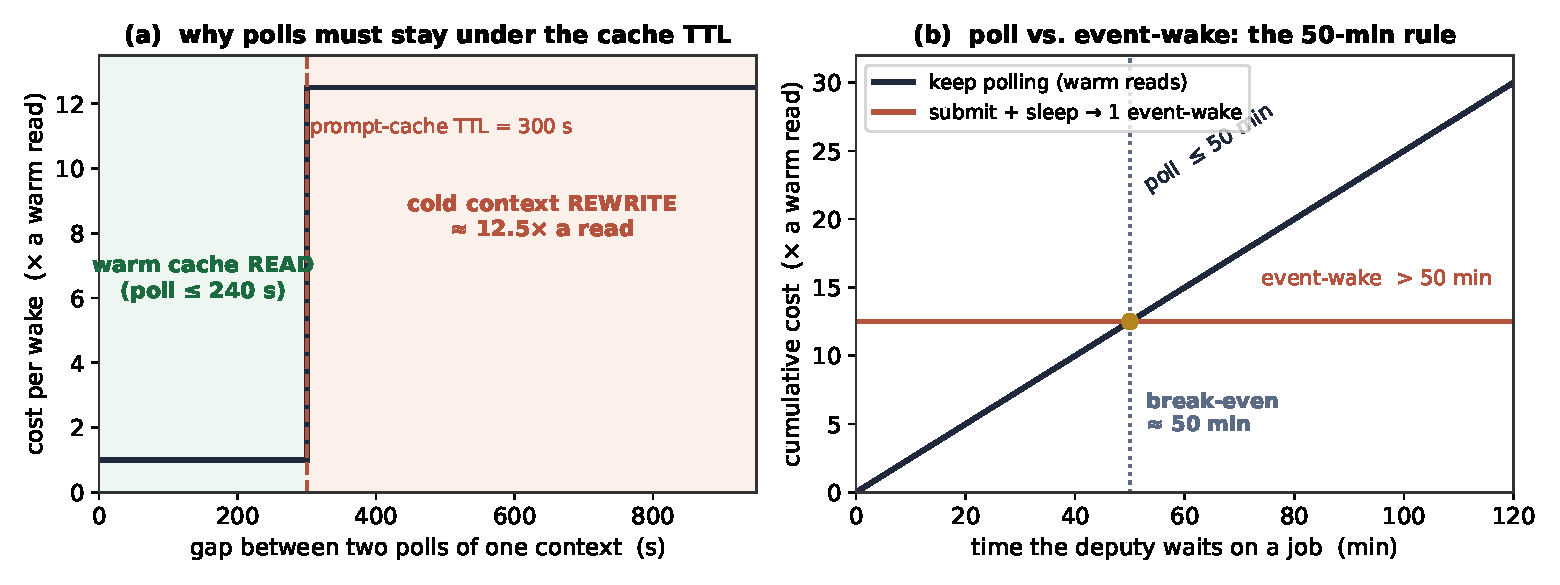
\includegraphics[width=0.99\columnwidth]{fig/fig_costmodel.pdf}
\caption{The cost model behind Posse's wait policy (a \emph{schematic} of the economics,
not a trace of measured traffic). (a) A poll within the cache TTL is a warm read; past
it, a cold rewrite at $\sim$12.5$\times$. (b) Cumulative cost of waiting: repeated warm
polls grow with duration, one event-wake is a single cold rewrite; they cross at
$\sim$50\,min --- the threshold between the two strategies.}
\label{fig:cost}
\end{figure}

\noindent\textbf{The policy.} Two rules fall out. \textbf{(1) Short waits: poll under
the TTL.} Sleep in chunks shorter than the TTL so every wake is a warm read.
\textbf{(2) Long waits: submit and sleep.} Hand the wait to a zero-API job manager and
\emph{end the turn}; the manager wakes the deputy by \emph{event} when the job finishes
--- one cold rewrite, once --- rather than paying a warm read every few minutes for an
hour.

\insight{The break-even, in closed form.}{Under three assumptions --- (a) each poll is
itself a cache-\emph{touch} that renews the TTL, and the cadence is set below the TTL
(e.g.\ $\le$240\,s under a 300\,s TTL, the margin absorbing jitter) so the \emph{next}
poll lands inside the window the current one opened; (b) an event-wake is one cold
rewrite plus $O(1)$ bookkeeping; (c) cost is linear in the number of touches --- the
accounting is simple. Let $m$ be the rewrite-to-read multiplier and $r$ the warm polls
per hour at that cadence. Polling for a wait of $t$ \emph{hours} costs $\approx r\,t$
reads; an event-wake costs $\approx m$ reads. The break-even is $t^{\star}\approx m/r$.
Crucially, \emph{context size cancels} --- both a read and a rewrite scale with it --- so
under this model $t^{\star}$ is independent of how large the thread has grown, and one
threshold is correct for every deputy. For $m\approx 12.5$ and $r\approx 15$ (a poll per
$\sim$4\,min under a 5-minute TTL), $t^{\star}\approx 50$\,min (Fig.~\ref{fig:cost}b).}

\noindent\textbf{Two more cost levers.} (i) \emph{Zero-API control plane (I3)}: every
always-on daemon runs without an LLM call, so only real work and rare manager decisions
are billed. (ii) \emph{Model tiering}: cheaper-but-capable models run token-heavy
domains and every Sheriff call; capable models run the rest, as a per-precinct default.

\insight{Why this generalizes.}{The constants are provider-specific, but the principle
generalizes to any backend with a \emph{TTL-bounded} read/rewrite discount: there is a
break-even $m/r$ between ``keep the context warm'' and ``tear down and event-wake.''
(Backends with a persistent cache or a per-write surcharge change or remove it, and need
the model re-derived.) Prompt-cache economics are heavily exploited at the
\emph{inference-serving} layer --- prefix sharing and KV-cache
reuse~\cite{vllm,sglang,gimcache} and provider prompt caching~\cite{promptcache,openaicache};
to our knowledge they have not been lifted into an \emph{agent scheduler's} wait/park
decision, and we would welcome pointers to prior work.}

% ======================================================================
\section{Analytical Evaluation}
\label{sec:eval}
% ======================================================================
We evaluate the cost policy \emph{analytically} --- from the model of
\S\ref{sec:cost}, not from a benchmark against other systems (a fair one is hard across
regimes, \S\ref{sec:related}). Figure~\ref{fig:eval} instantiates the model for a fleet
whose job-wait durations span a heavy-tailed mix (many short waits, a few multi-hour
jobs). Panel (a) plots per-wait cost for three policies --- a \emph{cost-unaware} coarse
cadence (every poll a cold rewrite), \emph{sub-TTL polling} alone, and \emph{Posse}
(poll while short, event-wake past $t^{\star}$). Posse is the lower envelope: it inherits
sub-TTL polling's cheap short waits and caps the long tail at a single rewrite. Panel (b)
aggregates over the mix: relative to Posse, the cost-unaware policy spends
$\sim$8.9$\times$ and sub-TTL-polling-alone $\sim$1.8$\times$ --- the coarse-cadence
factor being the analytical analog of the cost regression noted in \S\ref{sec:cost}.
These are model predictions, clearly labelled as such; an empirical study --- a live cost
microbenchmark, a fault-injection test of the interrupt/recovery invariants
(\S\ref{sec:email}), and a longitudinal fleet trace --- is the natural next step, and the
present paper's main threat to validity (\S\ref{sec:related}).

\begin{figure}[t]
\centering
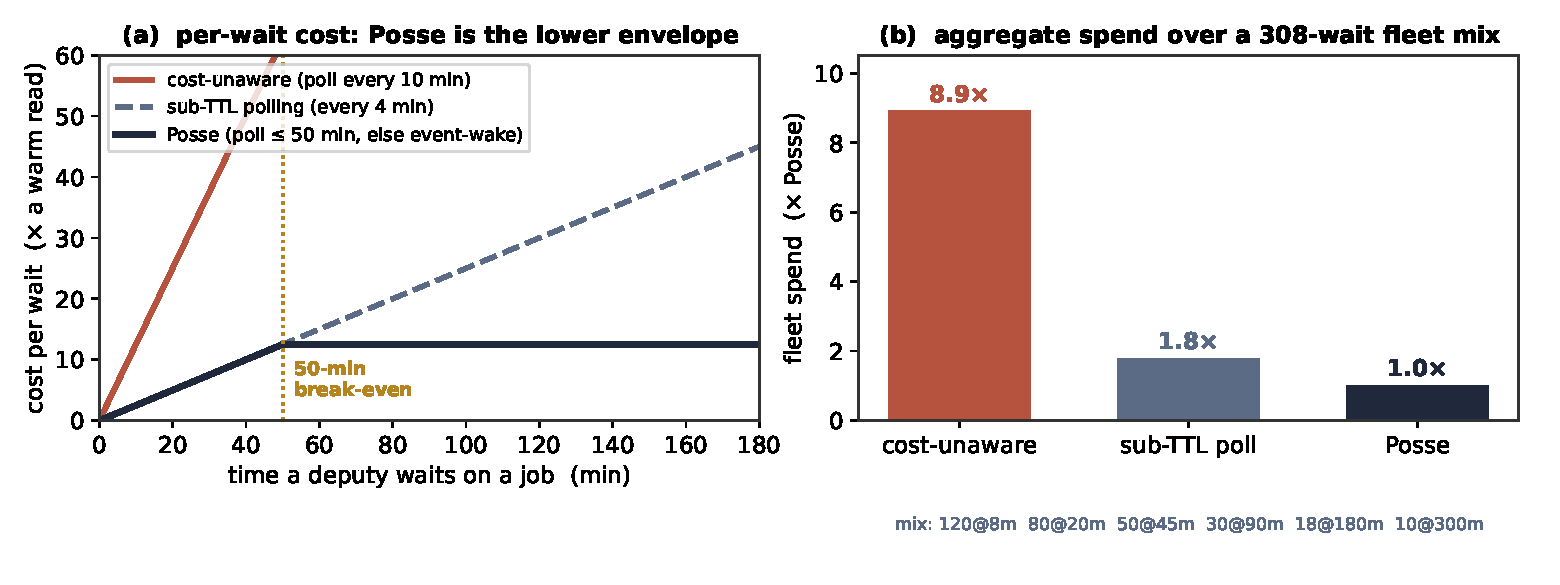
\includegraphics[width=0.99\columnwidth]{fig/fig_eval.pdf}
\caption{Analytical cost of the wait policy over a heavy-tailed fleet job-mix. (a)
Per-wait cost: Posse is the lower envelope of sub-TTL polling and event-wake. (b)
Aggregate fleet spend relative to Posse: a cost-unaware coarse cadence spends
$\sim$8.9$\times$, sub-TTL polling alone $\sim$1.8$\times$. Model-derived, not measured.}
\label{fig:eval}
\end{figure}

% ======================================================================
\section{Multi-Agent Coordination}
\label{sec:jtf}
% ======================================================================
\textbf{Role (R3).} Most cases are one deputy; four primitives handle work that is not.
The orchestrator-worker and hand-off shapes are standard~\cite{swarm,autogen}; what is
specific to Posse is that they operate over \emph{durable identities}, so a hand-off or a
wait must respect the identity/continuity machinery of \S\ref{sec:deputies}.
\begin{itemize}[leftmargin=1.1em,itemsep=1.5pt,topsep=2pt]
  \item \textbf{Sub-deputies.} A deputy spawns a tracked child for a sub-task, numbered as
  a child of the parent case, so a large effort decomposes into a \emph{visible} tree
  rather than an opaque recursion.
  \item \textbf{Manager-wake on completion.} A parent waiting for children does not
  busy-wait (which would burn context, I2); it registers ``wake me when $X$ finishes''
  and parks, and the Sheriff wakes it when the children's done-markers appear --- the
  event-wake idea (\S\ref{sec:cost}) applied to inter-agent dependencies.
  \item \textbf{Joint task forces.} For work needing several agents at once, a lead plus
  collaborators (and an optional critic) are assembled; each slot is either a precinct
  (spawn a fresh deputy) or a specific deputy (a ``must-take'' assignment).
  \item \textbf{Stop, hand over, then take} (the novel rule). Assigning work to a deputy
  already busy on another case would interleave two live cases in one linear context. Our
  rule --- chosen over ``refuse if busy'' and ``switch now'' --- has the busy deputy hand
  its current case to a new deputy with full context injected (reusing
  \S\ref{sec:deputies}), then take the new role as a fresh case, so a durable identity is
  never forced to run two live cases at once.
\end{itemize}
A throwaway \emph{anonymous} worker --- most often a critic reviewing a draft --- files no
records and is owned solely by its spawner, keeping the tracked record clean while
enabling adversarial self-review.

% ======================================================================
\section{Observability}
\label{sec:dash}
% ======================================================================
\textbf{Role (R3).} A read-only dashboard renders the fleet for the human: the
case-lineage forest (which case followed which), the active-deputy board, job state,
Sheriff health, and each precinct's records. It is deliberately \emph{read-only over the
same records the system runs on} --- it computes nothing the system does not already
persist --- so it can never disagree with reality or perturb it; the persisted lineage
map (\S\ref{sec:deputies}) makes the view authoritative rather than reconstructed. This
is the reconciliation / desired-state pattern of cluster controllers~\cite{borg,k8s},
applied to an agent fleet.

% ======================================================================
\section{Discussion, Related Work, and Limitations}
\label{sec:related}
% ======================================================================
\textbf{Positioning.} Posse borrows freely: its deputies are ReAct-style
tool-agents~\cite{react}; its coordination echoes role-based multi-agent
work~\cite{autogen,metagpt,crewai}; its ledger compaction is a coarse cousin of MemGPT's
paging~\cite{memgpt} and Generative Agents' reflection~\cite{genagents}; and its
``LLM-as-managed-process'' stance is the one AIOS~\cite{aios} argues for. Its
\emph{systems} lineage is older still: the Sheriff's supervise-and-relaunch loop is a
supervision tree in the Erlang/OTP ``let it crash'' tradition~\cite{otp,actor}; the
read-only dashboard is a reconciliation / self-healing-controller pattern~\cite{borg,k8s};
and durable identity that survives process death is what durable-execution
engines~\cite{temporal,stepfns} (and, more weakly, DAG schedulers like
Airflow~\cite{airflow}) give ordinary workflows. The newer harness/runtime layer is complementary, not
competing: a meta-harness like Omnigent~\cite{omnigent} or exo~\cite{exo} is exactly the
kind of backend a deputy could run \emph{inside}, and a secured runtime like
NemoClaw~\cite{nemoclaw} or OpenHands~\cite{openhands} is where a deputy's process could
be sandboxed; Posse is the layer \emph{above} them that gives the fleet durable identity,
async human steering, self-recovery, and cost scheduling. Job schedulers
(Slurm~\cite{slurm}) and distributed actor runtimes (Ray~\cite{ray}) likewise submit,
wait on, and event-complete long tasks, but they schedule \emph{compute} without a
token-cost model or a durable LLM-thread identity. Observability
platforms~\cite{langfuse,agentops,phoenix} are the read-only counterpart to Posse's
dashboard --- Posse additionally \emph{acts} on what it sees. The contribution we could
not place in prior work is on the \emph{cost} axis: lifting the inference layer's
cache-TTL economics~\cite{vllm,sglang}~(\S\ref{sec:cost}) into an agent scheduler's
wait/park decision.

\noindent\textbf{Failure modes and open risks.} Four risks are inherent to the design.
(i) \emph{The Sheriff is a single point of failure} --- it is a root daemon restarted by
an idempotent supervisor, not itself watched by a peer; a silently-dead Sheriff halts
compaction and recovery until a human notices. (ii) \emph{Unsupervised work quality.}
Posse keeps deputies alive and cheap; it does not judge whether their output is
\emph{correct}. A deputy can do the wrong thing for a long time before the human reads
its message --- quality gating is orthogonal and out of scope. (iii)
\emph{Interrupt-race correctness.} The at-least-once idempotent drain (\S\ref{sec:email})
is the invariant that makes concurrent interrupts safe; a bug there reintroduces lost or
duplicated feedback, so this path needs the care of any lock protocol. (iv)
\emph{Compaction fidelity.} LLM compaction can drop or distort a case despite a
forbidding prompt; on a failed compaction the Sheriff waits and retries rather than
truncating, so a bad compaction is never \emph{committed} mechanically --- but a
successful-yet-imperfect one can still lose fidelity, with the never-compacted case log
as the backstop of record. The price is that a \emph{prolonged} compaction outage lets
the ledger sit over budget until a clean compaction succeeds (\S\ref{sec:sheriff}).

\noindent\textbf{Limitations.} (1) Posse targets a single-provider, single-operator
deployment; the cost constants are provider-specific and multi-tenant fairness is out of
scope. (2) We evaluate the design analytically and by construction, not against a
controlled benchmark of other systems --- a fair comparison is hard precisely because
they target different regimes. (3) The continuity threshold and several policies are
hand-tuned; learning them is future work. (4) Mechanical routing (I3) is less flexible
than an LLM router for genuinely ambiguous messages --- we accept occasional Receptionist
hand-offs as the price of predictability.

% ======================================================================
\section{Conclusion}
% ======================================================================
Agent frameworks have largely solved the inside of a task. As deployments grow into
long-running fleets, the binding constraint moves outside it: keeping many agents
working, cheaply, for a long time, under a human who steers but cannot supervise. Posse
is an operating system for that regime. Four decisions carry it --- identity decoupled
from process liveness, token cost as a scheduled resource, a zero-cost mechanical
control plane separated from paid cognition, and memory as a shared record rather than a
private context --- and together they turn continuity, concurrency, autonomy, cost, and
cross-agent knowledge transfer from failure modes into engineered system properties.
The Sheriff watches; the deputies work; the records remember; and the cost stays bounded
by design.

% ----------------------------------------------------------------------
\begin{thebibliography}{99}
\small
\bibitem{autogpt} Significant Gravitas. \emph{AutoGPT}. 2023.
\url{https://github.com/Significant-Gravitas/AutoGPT}.
\bibitem{babyagi} Y.\ Nakajima. \emph{BabyAGI}. 2023.
\url{https://github.com/yoheinakajima/babyagi}.
\bibitem{react} S.\ Yao et al. \emph{ReAct: Synergizing Reasoning and Acting in Language
Models}. ICLR, 2023.
\bibitem{reflexion} N.\ Shinn et al. \emph{Reflexion: Language Agents with Verbal
Reinforcement Learning}. NeurIPS, 2023.
\bibitem{tot} S.\ Yao et al. \emph{Tree of Thoughts}. NeurIPS, 2023.
\bibitem{gptresearcher} A.\ Elovic et al. \emph{GPT-Researcher: Autonomous Agent for
Deep Research}. 2023. \url{https://github.com/assafelovic/gpt-researcher}.
\bibitem{genagents} J.\ S.\ Park et al. \emph{Generative Agents: Interactive Simulacra
of Human Behavior}. UIST, 2023.
\bibitem{autogen} Q.\ Wu et al. \emph{AutoGen: Multi-Agent Conversation Framework}.
arXiv:2308.08155, 2023.
\bibitem{camel} G.\ Li et al. \emph{CAMEL: Communicative Agents for LLM Society}.
NeurIPS, 2023.
\bibitem{metagpt} S.\ Hong et al. \emph{MetaGPT: Meta Programming for a Multi-Agent
Collaborative Framework}. ICLR, 2024.
\bibitem{chatdev} C.\ Qian et al. \emph{Communicative Agents for Software Development
(ChatDev)}. ACL, 2024.
\bibitem{crewai} J.\ Moura et al. \emph{CrewAI}. 2023.
\url{https://github.com/crewAIInc/crewAI}.
\bibitem{langgraph} LangChain. \emph{LangGraph: Stateful, Multi-Actor LLM
Applications}. 2024. \url{https://github.com/langchain-ai/langgraph}.
\bibitem{swarm} OpenAI. \emph{Swarm: Lightweight Multi-Agent Orchestration}. 2024.
\url{https://github.com/openai/swarm}.
\bibitem{omnigent} Omnigent. \emph{Omnigent: Open-Source AI Agent Framework and
Meta-Harness}. 2024. \url{https://github.com/omnigent-ai/omnigent}.
\bibitem{exo} exo. \emph{exo: Agent Harness}. 2024.
\url{https://github.com/exoharness/exo}.
\bibitem{nemoclaw} NVIDIA. \emph{NemoClaw: Running Agents Securely in NVIDIA OpenShell
with Managed Inference}. 2025. \url{https://github.com/NVIDIA/NemoClaw}.
\bibitem{openhands} All Hands AI. \emph{OpenHands: An Open Platform for AI Software
Developers}. 2024. \url{https://github.com/All-Hands-AI/OpenHands}.
\bibitem{langfuse} Langfuse. \emph{Langfuse: Open-Source LLM Engineering and
Observability}. 2023. \url{https://github.com/langfuse/langfuse}.
\bibitem{agentops} AgentOps. \emph{AgentOps: Agent Observability and Cost Tracking}.
2024. \url{https://github.com/AgentOps-AI/agentops}.
\bibitem{phoenix} Arize AI. \emph{Phoenix: LLM/Agent Observability}. 2023.
\url{https://github.com/Arize-ai/phoenix}.
\bibitem{claudecode} Anthropic. \emph{Claude Code and the Claude Agent SDK}. 2024--2026.
\bibitem{assistants} OpenAI. \emph{Assistants API: Persistent Threads for Agents}.
2023--2024.
\bibitem{aios} K.\ Mei et al. \emph{AIOS: LLM Agent Operating System}. arXiv:2403.16971,
2024.
\bibitem{memgpt} C.\ Packer et al. \emph{MemGPT: Towards LLMs as Operating Systems}.
arXiv:2310.08560, 2023.
\bibitem{temporal} Temporal Technologies. \emph{Temporal: Durable Execution}. 2020--.
\url{https://temporal.io}.
\bibitem{stepfns} Amazon Web Services. \emph{AWS Step Functions}. 2016.
\bibitem{airflow} M.\ Beauchemin et al. \emph{Apache Airflow}. 2015.
\bibitem{otp} J.\ Armstrong. \emph{Making Reliable Distributed Systems in the Presence
of Software Errors}. PhD thesis, KTH, 2003.
\bibitem{actor} C.\ Hewitt et al. \emph{A Universal Modular ACTOR Formalism for
Artificial Intelligence}. IJCAI, 1973.
\bibitem{borg} A.\ Verma et al. \emph{Large-scale Cluster Management at Google with
Borg}. EuroSys, 2015.
\bibitem{promptcache} Anthropic. \emph{Prompt caching} --- a 5-minute-TTL cache write is
priced at $1.25\times$ base input tokens (1-hour TTL $2\times$) and a cache read at
$0.1\times$. Claude Developer Platform documentation, 2024--2026.
\url{https://platform.claude.com/docs/en/build-with-claude/prompt-caching}.
\bibitem{openaicache} OpenAI. \emph{Prompt Caching in the API}. 2024.
\url{https://platform.openai.com/docs/guides/prompt-caching}.
\bibitem{gimcache} I.\ Gim et al. \emph{Prompt Cache: Modular Attention Reuse for
Low-Latency Inference}. MLSys, 2024.
\bibitem{vllm} W.\ Kwon et al. \emph{Efficient Memory Management for LLM Serving with
PagedAttention (vLLM)}. SOSP, 2023.
\bibitem{sglang} L.\ Zheng et al. \emph{SGLang: Efficient Execution of Structured
Language Model Programs (RadixAttention)}. NeurIPS, 2024.
\bibitem{k8s} The Kubernetes Authors. \emph{Kubernetes: Production-Grade Container
Orchestration (controllers / reconciliation)}. 2014--.
\bibitem{slurm} A.\ Yoo, M.\ Jette, M.\ Grondona. \emph{SLURM: Simple Linux Utility
for Resource Management}. JSSPP, 2003.
\bibitem{ray} P.\ Moritz et al. \emph{Ray: A Distributed Framework for Emerging AI
Applications}. OSDI, 2018.
\end{thebibliography}

\end{document}
